\documentclass[11pt]{article}
\usepackage[margin=1in]{geometry}
\usepackage{amsmath,amssymb,amsthm,booktabs,natbib,hyperref,graphicx}
\usepackage[T1]{fontenc}
\hypersetup{colorlinks=true,allcolors=blue}
\newtheorem{proposition}{Proposition}
\newtheorem{lemma}{Lemma}
\theoremstyle{definition}
\newtheorem{assumption}{Assumption}
\newtheorem{definition}{Definition}
\newcommand{\Fhat}{\widehat F}
\newcommand{\Dhat}{\widehat D}
\newcommand{\ahat}{\widehat a}
\newcommand{\ghat}{\widehat\gamma}
\newcommand{\tlo}{\underline t}
\newcommand{\alo}{\underline a}
\newcommand{\dlo}{\underline d}
\title{Predicting a latent population summary from survey estimates:\\
what the interval is sensitive to, and what that costs}
\author{}
\date{}
\begin{document}
\maketitle
\begin{abstract}
\noindent
A survey covering many regions produces one estimate for each. Those
estimates are then used to describe a place the survey did not cover: a region
newly added to a frame, or one too small to sample. That means separating real
variation between places from sampling error, and the sampling error is itself
estimated, from designs supplying few degrees of freedom. We ask what that
costs.

The answer is not about estimation accuracy. Competing methods can be given
exactly the same information about the unknown spread of the true values and
still report very different widths, because they differ in how strongly the
reported width reacts to being wrong about that spread. We define that reaction,
show it is weaker for a method that subtracts the sampling error than for methods
whose width is proportional to the square root of a variance bound, and prove an
exact identity relating the two. Three things follow. The number of places a
practitioner needs is far smaller than a requirement stated on the variance alone
implies, and this is a property of the problem, not of the estimator. Two methods can change places, one narrower in one survey
and wider in another, at a computable point. And in one matched case the width
ratio depends on nothing but the number of places and the error budget; we
recorded that prediction before testing it, and one of its three parts failed.

We then give an interval exploiting the weaker reaction, with a guarantee stated
under a normal model and a bound computed rather than searched for, and report
where it stops working. On three European Social Survey questions
across three rounds it is narrower than a comparable method in 44 of 45 configurations,
under stated approximations and with no claim about coverage.
\end{abstract}

\section{Introduction}

A survey programme covering many countries, regions or domains produces one
estimate of some summary per population per round. A second analysis then uses
those estimates to say something about a population the survey did not cover:
a region added to a sampling frame, a country joining a programme, a domain too
small to have been sampled. Call the target $\theta_{K+1}$, the latent summary of
that population, and the observed inputs $Y_1,\dots,Y_K$, the survey estimates
for the populations that were covered.

The obstacle is that each $Y_c$ carries sampling error. The spread of the $Y_c$
is larger than the spread of the $\theta_c$, so an interval calibrated on the
observed spread is too wide for the latent target. Removing the difference means
subtracting a design variance from a between-population variance, and the design
variances are themselves estimated---from stratified cluster designs with, in the
European Social Survey regions we analyse, a median of 22 to 29 degrees of
freedom per population.

Two literatures meet here and neither answers the question. Small-area
estimation treats the sampling variances as known and targets areas that were
sampled \citep{fay1979estimates,rao2015small}; where it treats them as estimated
it corrects the mean squared error of an \emph{in-sample} predictor
\citep{wang2003mse,rivest2003mse,you2006hierarchical,maiti2014,sugasawa2017}.
Recent conformal work reaches valid confidence intervals for in-sample areas
without estimating the sampling variances at all: \citet{zhang2026conformal}
target ``the unknown expectations of the in-sample outcomes \dots{} conditional
on the realised sample'', and their split conformal construction is, in their
words, ``easier to implement than the direct or EBLUP interval, because there is
no need at all to estimate the sampling variances'' (their \S3.4). That is an
argument for their target, not against ours: an interval for a population the
survey never covered cannot avoid separating the two scales. Conformal
prediction of a future \emph{unit} within an area \citep{bersson2024optimal} is
a third target again. Prediction for an out-of-sample area is standard
through synthetic estimation, and the linear mixed-model literature does supply
prediction intervals for targets containing a new random effect
\citep{chatterjee2008}---but with the sampling variances treated as known.

\paragraph{What this paper adds.} Not another way to smooth design variances, and
not a claim that conformal prediction is robust here; our exact inference rests
on a normal--$\chi^2$ model and we say so. The contribution is in two parts.

\emph{A result about the problem.} Section~\ref{sec:sensitivity} isolates the
scale elasticity and shows that it, rather than the quality of the scale
estimate, decides which construction is narrowest. The consequences are checkable
and we check them: the number of populations required is smaller by $\rho^{-4}$
than a criterion on the variance component implies; two constructions cross, at a
computable point; and for one matched pair the scale bound cancels entirely,
giving a width ratio that depends only on $K$ and the error budget. That last
prediction was registered before the experiment that tests it, and one of its
three registered claims was refuted---the constant, by an amount we locate.

\emph{A procedure that exploits it.} Section~\ref{sec:method} constructs an
interval whose sensitivity to the unknown scale is the damped one, carries the
uncertainty of an estimated variance structure rather than substituting a fitted
value, and is computable by a conservative bound rather than a search.

\paragraph{What we do not claim.} The guarantee is proved in a restricted normal
model. Under a complex design its conditions fail, measurably, and we report
where the procedure nonetheless behaves and where it does not. On real survey
data we report widths, inputs and diagnostics, and no coverage: the latent target
is unobserved and a held-out population's direct estimate is not a substitute for
it.

\section{Target, information, and what has to be estimated}\label{sec:target}

\subsection{The two objects}

Write $\theta_c$ for population $c$'s latent summary and $Y_c$ for its survey
estimate, taken as a deviation from a fixed centre. The observed and the latent
object are not interchangeable, and the paper keeps them apart throughout:
\begin{equation}\label{eq:decomp}
Y_c=\theta_c+e_c,\qquad \operatorname{Var}(\theta_c)=A,\qquad
\operatorname{Var}(e_c)=D_c ,
\end{equation}
with $D_c$ the design variance of the survey estimate. The \emph{design share}
\begin{equation}\label{eq:rho}
\rho_c^2=\frac{D_c}{A+D_c}\in[0,1)
\end{equation}
is the fraction of the observed dispersion that is sampling error. An interval
calibrated on the $Y_c$ covers a further \emph{survey estimate}; covering a
further \emph{latent summary} requires removing that fraction.

\subsection{The interval}

Fix an integer $m\le K$, write $\operatorname{ord}_m$ for the $m$th smallest of
$K$ numbers, and let $t=D/A$ be the scale ratio, taken common across populations
for this section. Standardising $Z_c(t)=Y_c/\sqrt{1+t}$, the interval is
\begin{equation}\label{eq:band}
B(t)=[-R(t),\,R(t)],\qquad
R(t)=\operatorname{ord}_m\{|Z_c(t)|\}_{c=1}^K=q\,\kappa,
\end{equation}
where $q=\operatorname{ord}_m\{|Y_c|\}$ and
$\kappa=(1+t)^{-1/2}=\sqrt{A/(A+D)}=\sqrt{1-\rho^2}$. Here $q$ is a
statistic---the radius the observed spread itself supplies---and $\kappa$ is the
factor carrying it to the latent scale.

\begin{lemma}[Base validity]\label{lem:rank}
If $\theta_{K+1},Z_1(t),\dots,Z_K(t)$ are exchangeable with a continuous
distribution, then $\Pr\{\theta_{K+1}\in B(t)\}=m/(K+1)$. Under
\eqref{eq:decomp} with equal design variances this holds exactly at the true $t$,
because $Z_c(t)$ and $\theta_{K+1}$ are then i.i.d.\ $N(0,A)$. Write
$\alpha_0=1-m/(K+1)$.
\end{lemma}

Everything that follows concerns one difficulty: $t$ is unknown, so the interval
is evaluated at a bound for it rather than at its value.

\subsection{What has to be known precisely, and it is not $A$}

\textbf{The band depends on the two scales only through their ratio $\kappa$},
and not on $A$ separately. Since $\widehat A$ and $\widehat{A+D}$ are built from
the same observed spread, their errors partly cancel, and to first order
\begin{equation}\label{eq:elasticity_kappa}
\frac{\operatorname{RSE}(\widehat\kappa)}{\operatorname{RSE}(\widehat{\sqrt A})}
=\sqrt{\frac{\rho^4\sigma_T^2+\sigma_D^2}{\sigma_T^2+\sigma_D^2}}
\ \longrightarrow\ \rho^2
\end{equation}
as the design variances become well determined, where $\sigma_T^2$ and
$\sigma_D^2$ are the variances of the estimated total and design scales. A
requirement stated on $\widehat A$ therefore overstates what the band needs by a
factor $\rho^{-4}$ in the number of populations. Simulation puts the realised
gain at 14 to 24 times at $\rho^2=0.2$ and 2.0 to 3.8 times at $\rho^2=0.5$,
against the predicted $\rho^{-4}$ of 25 and 4.

\subsection{Two axes, not one}

Writing $\sigma_D^2=2D^2/\nu_{\mathrm{tot}}$ for a design-variance estimate on
$\nu_{\mathrm{tot}}$ degrees of freedom, the requirement
$\operatorname{RSE}(\widehat\kappa)\le\varepsilon$ becomes
\begin{equation}\label{eq:twoaxis}
\boxed{\ \frac{1}{K-1}+\frac{1}{\nu_{\mathrm{tot}}}\ \le\
\frac{2\varepsilon^2(1-\rho^2)^2}{\rho^4}\ }
\end{equation}
Populations and design degrees of freedom enter \emph{harmonically}: neither
substitutes for the other, and $\nu_{\mathrm{tot}}$ imposes a floor no number of
populations clears. Replicate count does not help---with design degrees of
freedom $\nu^{\mathrm{des}}=20$, raising a resampling count from 100 to 10{,}000
buys 3.6 effective degrees of freedom and no more.

\paragraph{The boundary is not an artefact of this estimator.} Condition
\eqref{eq:twoaxis} is sufficient, and it was derived from one estimator's
relative standard error. A matching necessary condition holds. Restrict to equal
design variances and take two parameter points separated so that their
$\varepsilon$-balls in $\kappa$ are disjoint. The scaled-$\chi^2$ and normal
Hellinger affinities are available in closed form, so Le Cam's two-point bound \citep{lecam1986}
gives, exactly and in finite samples, that \emph{no} procedure can certify
$\kappa$ to tolerance $\varepsilon$ with failure probability $\eta<1/2$ unless
\begin{equation}\label{eq:necessary}
\nu_{\mathrm{tot}}\ \ge\ L(\eta)\,\frac{\rho^4}{\varepsilon^2(1-\rho^2)^2},
\qquad L(\eta)=-\log\big\{2\sqrt{\eta(1-\eta)}\big\},
\end{equation}
and the same bound with $K$ in place of $\nu_{\mathrm{tot}}$. The dependence on
$\rho$ and on $\varepsilon$ is the same as in \eqref{eq:twoaxis}; the constants
differ by a factor $2.4$ to $2.9$ over the range we checked ($\rho^2\ge0.4$,
$\varepsilon\le0.05$, $\eta=0.05$), one side being exact and the other a normal
approximation. At small design share the perturbation approaches the edge of the
parameter space and the bound loosens, to a factor $14$ at $\rho^2=0.2$,
$\varepsilon=0.05$.

The two axes carry the \emph{same} constant, and not by coincidence. Writing
$\tau$ for the ratio of the two $\kappa$ values, the $\nu$-axis perturbation
multiplies $D$ by $(1-\tau^2\kappa^2)/(1-\kappa^2)$ while the $K$-axis
perturbation multiplies $A+D$ by exactly its reciprocal, and the affinity
$\{2\sqrt r/(1+r)\}^{n/2}$ is invariant under $r\mapsto 1/r$. That is why the two
enter harmonically rather than in some other combination.

\emph{Neither the technique nor, in this submodel, the problem is new.} With
equal design variances the model is the balanced one-way random-effects model,
$\kappa$ is a monotone function of the intraclass correlation, exact intervals
for that coefficient are classical, and trading the number of groups against the
number of observations per group to control interval length is an established
design literature \citep{donner1986,zou2012icc,mondal2024review}. The
minimax theory for signal-to-noise ratios in high-dimensional regression
\citep{verzelen2018snr} concerns a different observation structure: there is no
separate channel carrying the error scale on a known number of degrees of
freedom, which is what produces the second axis here. We state
\eqref{eq:necessary} to establish that \eqref{eq:twoaxis} reflects the problem
rather than our estimator, and we claim nothing further for it.

\subsection{Estimating the design variances costs little; the estimator costs a lot}

Treating $D_1,\dots,D_K$ as unknown nuisance parameters observed through
$\nu_c\Dhat_c/D_c\sim\chi^2_{\nu_c}$, the effective information for $A$ is
\begin{equation}\label{eq:ieff}
I_{\mathrm{eff}}(A)=\tfrac12\sum_c\big\{(A+D_c)^2+D_c^2/\nu_c\big\}^{-1},
\end{equation}
so the standard error for $A$ inflates, relative to known design variances, by at
most $\sqrt{1+\rho^4/\nu_{\min}}$: 3.2\% at $\nu=10$ and $\rho^2=0.8$, 7.7\% at
$\nu=4$, 14.9\% at $\nu=2$. \textbf{At the degrees of freedom we examine, not
knowing the design variances is a second-order cost.} The bound is attained
exactly, in finite samples, by a moment estimator with weights
$w_c\propto\{(A+D_c)^2+D_c^2/\nu_c\}^{-1}$.

The first-order cost is the estimator. Under dispersed design variances the
unweighted subtraction $\widehat A=K^{-1}\sum_c(Y_c^2-\Dhat_c)$ has relative
efficiency 23\% against \eqref{eq:ieff}, where oracle weighting reaches 99\%. And
substituting $\Dhat_c$ into a known-variance likelihood biases $\widehat A$
\emph{upward} by approximately $4\rho^4/\{\nu(1-\rho^2)\}$ relative to $A$, a
bias of order $1/\nu$ that does not average away as populations accumulate. The
second-order mean-squared-error corrections of \citet{prasad1990} and
\citet{datta2000} address the same estimated-variance effect for an in-sample
predictor, where the target makes the correction additive rather than a
multiplicative distortion of a band.

These are properties of the estimation problem. What matters for the interval is
the next section.

\section{Scale sensitivity}\label{sec:sensitivity}

No construction evaluates its half-width at the truth. Each evaluates it at a
bound. \textbf{What separates constructions is therefore not how well they
estimate the scale---they can be given the same estimate---but how hard the
interval reacts to being wrong about it.}

\begin{definition}
For a half-width $R$ depending on a scale $\theta$, the \emph{scale elasticity}
is $e(\theta)=\partial\log R/\partial\log\theta$.
\end{definition}

\paragraph{What is held fixed.} The derivative is taken in the scale at which
the half-width is \emph{evaluated}, with the data---and hence the empirical
radius $q=\operatorname{ord}_m|Y_c|$ of \eqref{eq:band}---held fixed. It is not
the derivative of the oracle width: at the truth every construction here has
half-width proportional to $\sqrt A$ and so oracle elasticity $1/2$. The
distinction is the substance of this section. Constructions can be given the same
information about the scale and still differ in how an error in the plugged-in
bound propagates into the number they report, and it is that propagation, not the
quality of the estimate, that decides which is narrower.

With latent scale $A$ and design variance $L$, so $\rho^2=L/(A+L)$:

\begin{center}
\begin{tabular}{lll}
\toprule
construction & half-width & elasticity in $A$\\
\midrule
deconvolution band & $q\sqrt{A/(A+L)}$ & $L/\{2(A+L)\}=\rho^2/2$\\
any band $\propto\sqrt A$ & $z\sqrt A$ & $1/2$\\
uncorrected anchor & $q$ & $0$\\
\bottomrule
\end{tabular}
\end{center}

The deconvolution band's elasticity is \textbf{damped by the design share}. This
is not a property of conformal prediction: it follows from dividing by
$\sqrt{A+L}$ and multiplying by $\sqrt A$, and any construction of that form
inherits it.

Figure~\ref{fig:elasticity} shows both halves of the claim: the relative cost of
a loose bound on the left, and on the right the elasticity measured in eight
simulation cells against the predicted $\rho^2/2$. The measurement sits below
the prediction in every cell, averaging $0.86$ of it---the damping is real and is
slightly stronger than the first-order calculation says, which is the safe
direction for a claim of the form ``this construction reacts less''.

\begin{figure}[t]
\centering
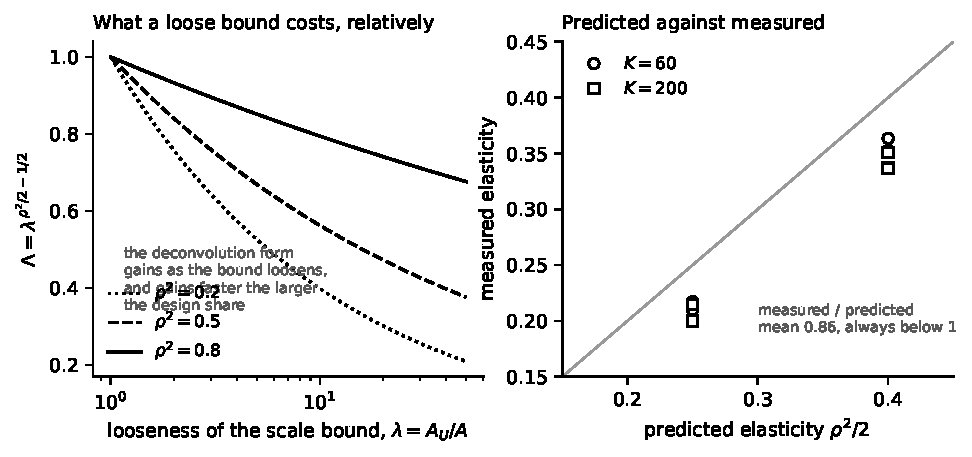
\includegraphics[width=\textwidth]{figures/fig1_elasticity}
\caption{\textbf{Left:} the exchange identity of
Proposition~\ref{prop:exchange}. Evaluated at a bound loose by $\lambda$, the
deconvolution band's half-width moves by $\lambda^{\rho^2/2}$ where a band
proportional to $\sqrt{A}$ moves by $\lambda^{1/2}$; the curves are their exact
ratio, with no fitted constant. \textbf{Right:} elasticity measured in eight
cells ($K\in\{60,200\}$, $\bar D/A\in\{1,4\}$, $\nu=10$) against the predicted
$\rho^2/2$. The line is equality.}
\label{fig:elasticity}
\end{figure}

\begin{proposition}[Exchange identity]\label{prop:exchange}
For the deconvolution band $R_c$ and any band $R_g\propto\sqrt A$, evaluated at a
common upper bound $A_U\ge A$,
\[
\frac{R_c(A_U)/R_g(A_U)}{R_c(A)/R_g(A)}=\sqrt{\frac{A+L}{A_U+L}}=:\Lambda .
\]
\end{proposition}
\begin{proof}
$R_c(A_U)/R_c(A)=\sqrt{A_U(A+L)/\{A(A_U+L)\}}$ and
$R_g(A_U)/R_g(A)=\sqrt{A_U/A}$; divide.
\end{proof}

The identity is exact, not asymptotic, and we verified it numerically on
$2\times10^5$ random $(A,L,A_U)$ with no violations. Its content: $\Lambda\to1$
as $L\to0$---with no design noise there is nothing to deconvolve and no
advantage---and $\Lambda\to\sqrt{A/A_U}$ as $L/A\to\infty$. \textbf{The
deconvolution form's advantage is bought entirely by design noise, and it is
largest exactly when the scale bound is loosest.}

\paragraph{Consequence 1: the requirement.} Certifying $\widehat A$ and
certifying the band's own scale factor to the same tolerance differ by the
elasticity ratio, and the population requirement by its square, $\rho^4$---the
saving reported in Section~\ref{sec:target}, where \eqref{eq:necessary} shows it
is a property of the problem and not of the estimator used to realise it.

\paragraph{Consequence 2: constructions cross.} Two forms with elasticities
$e_1<e_2$ and oracle width ratio $r_0$ realise $r_0\lambda^{e_1-e_2}$ at a bound
loose by $\lambda=A_U/A$, and cross at $\lambda^\star=r_0^{-1/(e_2-e_1)}$: below
it the higher-elasticity form is narrower, above it the lower one is. A single
pair of constructions therefore changes places between survey settings. Two of
our own experiments straddle that point---one finds the normal-theory band
narrower by 2 to 22\%, the other finds it wider by 7 to 14\%---and the
elasticity reconciles them, since the first uses a tight scale limit and the
second a loose one. \textbf{We do not present this as a measured crossing.} The
two runs differ in more than the tightness of the limit and the later supersedes
the earlier, so what the calculus supplies here is an explanation for a
disagreement we had previously recorded as an error, not an experiment designed
to locate $\lambda^\star$.

\paragraph{Consequence 3: sometimes the bound cancels.} If the comparator's bound
is built from the deconvolution band's own statistic---$A_U=\bar
S/\chi^2_{K,\alpha_2}$ with $\bar S=\sum_cY_c^2/(1+\tlo)$, against
$\operatorname{ord}_m|Y_c|/\sqrt{1+\tlo}$---then $\tlo$, $A$, $L$, $\rho$ and
$\nu$ all cancel:
\begin{equation}\label{eq:S4}
\frac{R_{\mathrm{deconv}}}{R_{\mathrm{normal}}}\ \approx\
\frac{z_p}{z_{1-\alpha_1/2}}\sqrt{\frac{\chi^2_{K,\alpha_2}}{K}},
\qquad p=\frac{m}{K+1}.
\end{equation}

\subsection{A registered test, and what it refuted}

Equation~\eqref{eq:S4} makes a strong claim: a ratio built entirely out of design
variances should not depend on the design share. We wrote the predicted values
into a protocol before running a fresh grid ($K\in\{40,120,400\}$,
$\rho^2\in\{0.20,0.45,0.70\}$, $\nu\in\{6,20\}$, correct and misspecified
structure; none of these values used in the experiment that suggested the law).

\begin{center}
\begin{tabular}{lccc}
\toprule
registered prediction & result & tolerance & verdict\\
\midrule
dependence on the error-budget split & error \textbf{identical to $10^{-6}$} across six splits & monotone, 5\% & \textbf{passes}\\
level of the ratio & worst cell \textbf{7.07\%} & 5\% & \textbf{fails}\\
invariance in $\rho^2$ and $\nu$ & within-$K$ spread 0.0200/0.0110/0.0089 & 0.02 & marginal\\
\bottomrule
\end{tabular}
\end{center}

The first row is the sharpest test and it passes exactly: across six splits
spanning a factor of $1.32$ in the predicted ratio, the discrepancy is one
constant. The second row locates that constant---$c(K)=1+1.9/K$, the order
$1/K$ gap between an order statistic's expectation and the corresponding
quantile---and the refined form errs by at most 2.2\%. The third row shows the
invariance is \emph{asymptotic}: a residual dependence on $\rho^2$ of 1.4\% at
$K=40$ falls to 0.45\% at $K=400$. \textbf{The strong form of the invariance
claim is refuted}, and what stands is a dependence an order of magnitude smaller
than the construction of the quantity would suggest.

\paragraph{Why this widens the comparison.} The elasticity is a property of the
\emph{form} $c\sqrt{\theta}$, not of a particular baseline. Any interval whose
half-width is proportional to the square root of a scale bound---a normal-theory
interval, an EBLUP prediction interval for a target containing a new random
effect, a parametric bootstrap interval built on one---has elasticity $1/2$ and
so pays the full $\lambda^{1/2}$ for scale uncertainty. Proposition
\ref{prop:exchange} therefore compares against a class rather than against a
single constructed competitor. \textbf{It does not rank them absolutely}: the
oracle ratio $r_0$ differs between constructions and is not supplied by the
elasticity. What the identity gives is the differential response to scale
uncertainty, which is the part that reverses.

\section{A procedure that exploits the damping}\label{sec:method}

Section~\ref{sec:sensitivity} says the interval should depend on the unknown
scale as weakly as it can while still covering. This section builds one that
does, and makes it an algorithm.

\subsection{Model}

\begin{assumption}[Model R]\label{as:R}
Independently across $c=1,\dots,K$, with $\mu$ known,
\[
Y_c\sim N(0,\,A+d\,a_c),\qquad
\frac{\nu_c\Dhat_c}{d\,a_c}\sim\chi^2_{\nu_c},\qquad Y\perp\Dhat,
\]
where $a_c>0$ is a \emph{relative} design-variance structure, $d>0$ an unknown
common scale, and $A>0$ the between-population variance. Write $t=d/A$, so that
$D_c/A=a_ct$: one unknown ratio parameter.
\end{assumption}

Assumption~\ref{as:R} is the heteroscedastic model in which reduction to one
ratio parameter is \emph{true} rather than assumed. A general heteroscedastic
model does not reduce this way, and substituting $\Dhat_c$ for $D_c$ to force it
would reintroduce exactly the fault the construction exists to avoid.

\subsection{An exact pivot for the correction ratio}

\begin{proposition}\label{prop:pivot}
Under Assumption~\ref{as:R}, with $\nu=\sum_c\nu_c$,
$\widehat d=\nu^{-1}\sum_c\nu_c\Dhat_c/a_c$ and
$S(t)=\sum_cY_c^2/(1+ta_c)$,
\[
T(t)=\frac{K\widehat d}{t\,S(t)}\ \sim\ F_{\nu,K}\quad\text{exactly},
\]
and $\partial_t\{tS(t)\}=\sum_cY_c^2/(1+ta_c)^2>0$, so $T$ is strictly decreasing
and inverts to an exact one-sided lower bound $t_L$, the solution of
$T(t_L)=f_{\eta_t}$ with $f_{\eta_t}$ the upper $\eta_t$ quantile of
$F_{\nu,K}$, satisfying $\Pr\{t\ge t_L\}=1-\eta_t$.
\end{proposition}

The band is \eqref{eq:band} with the heteroscedastic standardisation, so its
oracle half-width is
\[
R(t)=\operatorname{ord}_m\big\{|Y_c|/\sqrt{1+a_ct}\big\},
\]
and Lemma~\ref{lem:rank} applies at the true $t$ with $\alpha_0=1-m/(K+1)$.
Since $R(t)$ is
decreasing in $t$, $R(t_L)$ bounds it above on that event. \textbf{One parameter,
one budget, one bound}---against a construction that spends one budget on an
upper limit for $A$ and another on $K$ simultaneous lower limits for the $D_c$,
both of which drive the correction toward zero.

\subsection{An estimated structure, paid for rather than substituted}

With $a_c(\gamma)=x_c^{-\gamma}/\overline{x^{-\gamma}}$ for a design variable
$x_c$ known before any estimate is seen, write
$\epsilon_c=\log(\chi^2_{\nu_c}/\nu_c)$, whose law is known. The statistic
\[
W(\gamma)=\sum_c(\log x_c-\overline{\log x})\{\log\Dhat_c+\gamma\log x_c\}
\]
has, at the true $\gamma$, a null law depending on neither $d$ nor $\gamma$, and
is linear increasing in $\gamma$. Hence
\begin{equation}\label{eq:Cgamma}
C_\gamma=\Big[\ghat-\tfrac{w}{S_{xx}},\ \ghat+\tfrac{w}{S_{xx}}\Big],
\qquad \ghat=-S_{xD}/S_{xx},
\end{equation}
in closed form, with $\Pr\{\gamma_0\in C_\gamma\}\ge1-\eta_\gamma$. The interval
is then
\[
R_U=\sup_{\gamma\in C_\gamma}R\big(t_L(\gamma),\gamma\big),
\]
and on $\{\gamma_0\in C_\gamma\}\cap\{t\ge t_L(\gamma_0)\}$ it dominates the
oracle half-width, so
\begin{equation}\label{eq:guarantee}
\Pr\{\theta_{K+1}\notin B_U\}\ \le\ \alpha_0+\eta_\gamma+\eta_t .
\end{equation}
No independence between the two confidence events is required.

\subsection{Making the supremum a computation}

A grid maximum is not a supremum, and \textbf{we found by counterexample that the
minimiser of $t_L(\gamma)$ can be interior}, 16.9\% below the smaller endpoint,
so an endpoint evaluation is not available. A bound is.

\begin{lemma}\label{lem:concave}
$\partial_\gamma\log a_c(\gamma)=\bar\ell(\gamma)-\log x_c$ with
$\bar\ell'(\gamma)=-\operatorname{Var}_w(\log x)\le0$, so $\log a_c$ is concave in
$\gamma$ and
$\inf_{\gamma\in[\gamma_L,\gamma_U]}a_c(\gamma)=\min\{a_c(\gamma_L),a_c(\gamma_U)\}$
exactly.
\end{lemma}

\begin{proposition}[Certified bound]\label{prop:cert}
Let $\alo_c$ be that endpoint minimum and
$\bar\Phi(t)=\sum_ctY_c^2/(1+t\alo_c)\ \ge\ tS(t;\gamma)$ for every
$\gamma\in C_\gamma$. Since $1/a_c(\gamma)=K^{-1}\sum_j(x_c/x_j)^\gamma$ is a
positive sum of exponentials, $\widehat d(\gamma)$ is convex, and a bisection on
its increasing derivative brackets the minimiser, giving a certified $\dlo$.
Then
\[
\tlo=\bar\Phi^{-1}\big(K\dlo/f_{\eta_t}\big)\ \le\ \inf_{\gamma\in C_\gamma}t_L(\gamma),
\]
and $\operatorname{ord}_m\{|Y_c|/\sqrt{1+\tlo\alo_c}\}\ \ge\
R(t_L(\gamma),\gamma)$ for every $\gamma$ in the set.
\end{proposition}

The bound needs two structure evaluations, one convex minimisation and one
monotone inversion, which is cheaper than the grid it replaces. An optimiser's returned
value is not a lower bound and is not used: the endpoint cases are exact and the
interior case uses a supporting line at a certified bracket, with every returned
quantity shrunk by a relative $10^{-9}$ for rounding. Verified: no violations in
400 stress configurations, tightness median 0.941.

\paragraph{Unknown centre.} With $Y\sim N(X\beta,AI+\operatorname{diag}(\mathbf
D))$ and $\operatorname{rank}(X)=p$, refitting the weighted regression at each
candidate gives $Q(A,\mathbf D)=\min_\beta\sum_c(Y_c-x_c'\beta)^2/(A+D_c)\sim
\chi^2_{K-p}$, and the argument extends. \textbf{This bounds the variance
component only}: it says nothing about the error from centring the band on an
estimated mean, or about exchangeability of the scores under an estimated centre.
Both matter in Section~\ref{sec:ess}.

\section{Simulation: what holds, and where it stops}\label{sec:simulation}

Three questions, and the third is the one that decides whether the procedure is
worth using.

\subsection{Against a comparator sharing the target, information and level}

The direct comparator is a normal-theory prediction interval for the \emph{same}
new population's latent value, built from the \emph{same} structure confidence
set and the \emph{same} certified scale bound, spending the identical budget
$\alpha_0+\eta_\gamma+\eta_t=0.10$: $A_U=\bar S/\chi^2_{K,\alpha_2}$, the exact
chi-square limit rather than a Satterthwaite or \citet{graybill1980}
approximation \citep{satterthwaite1946}, and
$\pm z_{1-\alpha_1/2}\sqrt{A_U}$ with $\alpha_1+\alpha_2=\alpha_0$. The two arms
differ in exactly one place.

\begin{center}
\begin{tabular}{lcccc}
\toprule
$K$ & proposed cov. & comparator cov. & \textbf{proposed narrower by} & split\\
\midrule
60 & 0.957--0.978 & 0.982--0.996 & 22.2\% & scanned in its own favour\\
60 & --- & --- & \textbf{25.9\%} & fixed in advance\\
200 & 0.957--0.970 & 0.983--0.988 & 13.9\% & scanned in its own favour\\
200 & --- & --- & \textbf{20.4\%} & fixed in advance\\
\bottomrule
\end{tabular}
\end{center}

All against a guaranteed 0.90. The pre-registered split is the primary
comparison; the scanned one gives the comparator its best budget allocation and
is the smaller number, so \textbf{we quote 13.9 to 22.2\% throughout}. Two
readings follow. Both arms over-cover, but the proposal is \emph{both} narrower
and closer to the nominal level, at 0.957--0.978 against 0.982--0.996: the width
difference is not bought by spending coverage. And the comparator is one valid
construction, not a class and not the best possible---the registered prediction
before this experiment was that it would win, and it did not.

\paragraph{A disagreement between two of our own runs.} On a tight scale limit
the normal-theory band is narrower by 2 to 22\% in eight cells; on a loose pivot
limit an earlier run found it wider by 7 to 14\%. We recorded the second as an
error and superseded it. Consequence~2 of Section~\ref{sec:sensitivity} says the
two are the two sides of $\lambda^\star$ and neither need be wrong. We report
this as a reconciliation and not as evidence: the runs differ in more than the
tightness of the limit, and an experiment that varies only $\lambda$ and locates
the crossing is one we have not done.

\subsection{The regimes where it stops}

Under finite-population stratified cluster sampling with a pre-specified
sample-size structure variable, the picture divides not by design share but by
what else changes with it.

\begin{center}
\begin{tabular}{lcc}
\toprule
& degrees of freedom 12--28 & degrees of freedom 4--8\\
\midrule
structure $R^2$ & 0.59--0.85 & 0.05--0.71\\
zero variance estimates & none & up to 17\%\\
\textbf{containment} & \textbf{0.955--0.992} & \textbf{0.681--0.987}\\
latent coverage & 0.958--0.971 & 0.944--0.975\\
band vs.\ structure-free & 0.883--0.937 & 0.836--0.928\\
\bottomrule
\end{tabular}
\end{center}

At matched $\bar D/A\in\{0.55,0.75\}$ the two columns differ in degrees of
freedom, in the rate of exactly-zero variance estimates and in the fit of the
structure model---\textbf{the same noise ratio is not the same inference
problem}. In the first column the procedure holds its containment requirement and
is 6.3 to 11.7\% narrower than a structure-free construction, capturing 0.56--0.74
of the available narrowing against 0.23--0.30. In the second it loses containment
at a tail quantile and its width figures are not usable.

Supplying the \emph{true} structure raises containment there from 0.68 to 0.82
and from 0.77 to 0.89 and does not reach 0.95. Two conclusions and only two:
approximating the variance structure affects the outcome, and improving that step
alone would not repair the procedure. We do not apportion the residue among
normality, the $\chi^2$ law and independence; this design breaks all three at
once and the experiment does not separate them.

\paragraph{We report the verified scenario range, not a usage threshold.} Writing
``degrees of freedom above 12 and structure $R^2$ above 0.6'' as an operating rule
would be wrong three times: those numbers co-occurred in these scenarios rather
than being derived as thresholds; the structure $R^2$ is computed from the
\emph{true} design variances and is unavailable in real data; and nothing here
proves normality or the $\chi^2$ law under any complex design.

\subsection{Honest accounting of the gain}

At the regional design share the \emph{valid} interval is 0.9 to 6.6\% narrower
than not correcting at all, capturing 6 to 31\% of what the oracle achieves. The
reason is the guarantee itself: the argument needs $A$ bounded above and each
$D_c$ bounded below, and both drive the correction toward zero. Measuring where
the width goes shows the simultaneity correction is only 6 to 22\% of that loss,
so replacing it alone would not repair matters---which is why the construction
bounds the ratio rather than the components.

\section{European Social Survey}\label{sec:ess}

\subsection{What the data can and cannot show}

The latent $\theta_{K+1}$ is unobserved. \textbf{No coverage is claimed or
computed here}, and a held-out region's direct estimate is not a substitute for
the latent value: treating it as one would measure the uncorrected anchor. What
real data can show is which inputs each construction needs, how far the intervals
differ on the same data, and which assumptions the data support.

\subsection{Design}

Rounds 9--11, 127{,}286 respondents, 75 country-rounds, 825 region-rounds,
retrieved through the portal API so that the analysis reproduces from source for
any user with an End User Licence. Everything was fixed before any estimate was
computed: the target is a single CDF point $F_{cr}(t_0)$ with $t_0$ set by rule
(one below the scale midpoint); three items chosen in advance for differing
between-region heterogeneity; the structure variable $x_{cr}$ is the region's
sampled PSU count, carried over unchanged from the simulations; one budget for
every arm; the comparator's split fixed rather than scanned. Regions with fewer
than two design degrees of freedom (18 of 825) are excluded and counted; regions
with a zero variance estimate (13, 39, 55 by item) receive no shrinkage, which is
conservative.

\subsection{The score and its variance must match}

The score is $Y_{cr}=\Fhat_{cr}-\Fhat_c$, a deviation from an \emph{estimated}
country centre. Its design variance is not that of $\Fhat_{cr}$: it is that of the
difference, and we compute it from the Taylor linearisation
\[
u_i=\frac{w_i\mathbf 1\{i\in r\}(z_i-\Fhat_{cr})}{W_r}-\frac{w_i(z_i-\Fhat_c)}{W_c}
\]
aggregated to PSU totals over the whole country-round. \textbf{This is not a
technicality.} With the wrong variance the fitted structure exponent has median
$0.53$ and its confidence set contains the elementary value $\gamma=1$
($D\propto1/n$) in \emph{none} of 45 configurations, including one implausible
negative estimate; with the right one the median is $1.14$ and the set contains
$\gamma=1$ in 17 of 45.

\subsection{What the arms do on the same data}

\begin{center}
\begin{tabular}{lcc}
\toprule
comparison & range over 45 configurations & \\
\midrule
proposed / normal-theory comparator & 0.729--1.014 & narrower in \textbf{44 of 45}, median 0.821\\
proposed / structure-free & 0.459--1.034 & narrower in 43 of 45, median 0.830\\
proposed / uncorrected & 0.422--0.867 & median 0.730\\
\bottomrule
\end{tabular}
\end{center}

\begin{figure}[t]
\centering
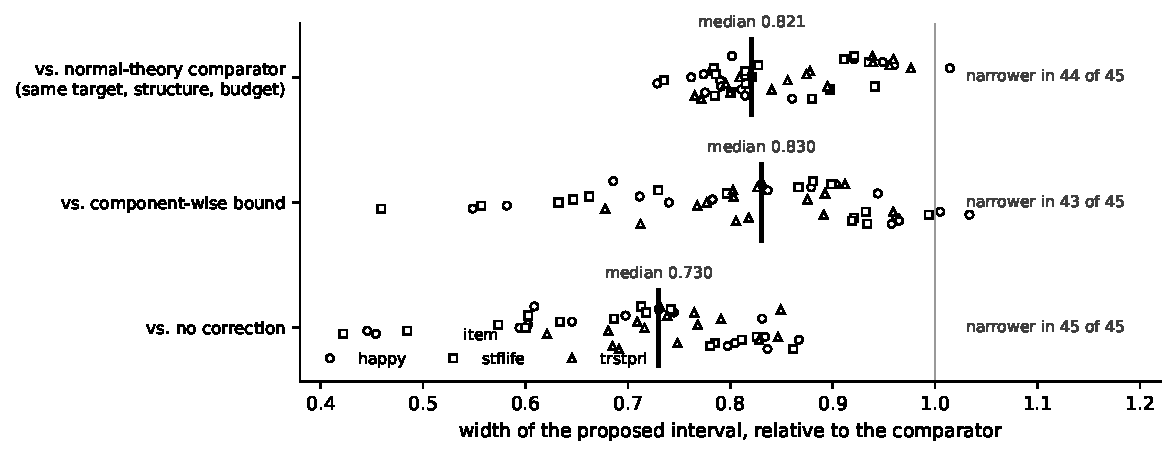
\includegraphics[width=\textwidth]{figures/fig2_ess_widths}
\caption{Width of the proposed interval relative to each comparator, over the 45
item-by-round-by-country configurations of European Social Survey rounds 9--11.
Bars are medians. All three comparisons use the variance of the centred score
(Section~\ref{sec:ess}); with the uncorrected variance the middle comparison
moves to a median of $0.992$. \textbf{No coverage is claimed}: the latent target
is unobserved.}
\label{fig:ess}
\end{figure}

The comparison against a comparator sharing the target reproduces the simulation
on real data---median 0.821 against a simulated 13.9--22.2\% reduction---and is
the robust one, because both arms are built on the same variance. Realised design
shares are $\widehat\rho^2\in[0.22,0.61]$: the regime the correction is for.

\subsection{Which assumptions the data support}

The pivot needs normality of the standardised regional deviations. Skewness and
excess kurtosis are $-0.47$ to $0.62$ and $0.3$ to $4.4$ for the first item, and
reach $2.30$ and $12.6$, and $2.81$ and $17.6$, for the other two.
\textbf{The condition is reasonably supported for one item of the three and
clearly not for the others}, and we report that with their results.

The structure model explains 0.09 to 0.23 of $\log\Dhat$ once the right variance
is used---moderately at best.

\paragraph{This is not the quantity that separated the two columns of
Section~\ref{sec:simulation}, and the two must not be compared.} There the
structure $R^2$ was computed against the \emph{true} design variances, which a
simulation supplies and a survey does not; here it is computed against estimated
ones, and estimation noise in $\log\Dhat$ depresses it by an amount we cannot
remove. A reader should therefore not conclude from $0.09$--$0.23$ that these
data sit in the regime where the procedure lost containment---nor that they sit
in the safe one. The honest statement is that the diagnostic available on real
data does not identify which column a real survey belongs to, and supplying that
mapping would require knowing the design variances one is trying to estimate. An analyst can compute that quantity, and across
these 45 configurations it is associated with whether using the structure pays
(correlation $-0.30$). \textbf{We report this as an observable exploratory
diagnostic and not as a criterion}: both quantities are built from the same
variance estimates so part of any association is arithmetic, and a good structure
fit does not imply coverage, which is not measured here.

\subsection{The approximation this analysis rests on}

Correcting the variance does not restore exchangeability. A common estimated
centre makes the scores dependent, and we measure it: the mean within-country
correlation among distinct regions is $-0.232$, $-0.116$, $-0.046$, $-0.029$ for
country-rounds with at most 5, 6--10, 11--20 and more than 20 regions---almost
exactly $-1/(n_r-1)$, the classical dependence of deviations from a common mean.
It is negative, hence the benign direction for a maximum-based rank statistic,
and it shrinks with the number of regions, but it is not zero.

\begin{quote}
\textbf{Status of this analysis.} An application of the procedure under a stated
approximation: the centre is estimated rather than known, and the scores carry a
measured dependence of about $-1/(n_r-1)$. \textbf{The guarantee of
Section~\ref{sec:method} is not attached to it.}
\end{quote}

\section{Discussion}\label{sec:discussion}

\subsection{Why a reader would use this, and on what evidence}

The question a reader brings is why to use this rather than what they already
have. The answer is in three parts and each has a different kind of support
behind it.

\emph{Because the quantity you must pin down is not the one you think.} The
interval depends on the two scales only through their ratio, and a requirement
stated on the variance component overstates what the band needs by $\rho^{-4}$ in
the number of populations. This is algebra, verified numerically, and it applies
whatever construction is used. It is also, by \eqref{eq:necessary}, a property of
the problem: the same $\rho^4/\{\varepsilon^2(1-\rho^2)^2\}$ appears in a
two-point lower bound on \emph{any} procedure that certifies the ratio, within a
factor of about $2.5$ of what our estimator achieves.

\emph{Because how an interval reacts to scale uncertainty is a property of its
form, and forms differ.} Proposition~\ref{prop:exchange} is exact, and it says
the deconvolution form pays $\lambda^{\rho^2/2}$ where every construction
proportional to a square-root scale bound pays $\lambda^{1/2}$. That covers a
class---normal-theory intervals, EBLUP prediction intervals for a target with a
new random effect, parametric bootstrap intervals built on them---rather than one
comparator. \textbf{It does not rank them absolutely}: the oracle width ratio
differs between constructions and the elasticity does not supply it. What it
supplies is the part that reverses, and the reversals are what a practitioner
would otherwise experience as unpredictability.

\emph{Because the resulting procedure is computable and its cost is measured.}
Under Assumption~\ref{as:R} it has the guarantee~\eqref{eq:guarantee}, the
supremum is bounded rather than searched, and against a comparator sharing the
target, information and level it is 14 to 22\% narrower in simulation and
narrower in 44 of 45 real survey configurations.

\subsection{What is not established}

\paragraph{The gap between the theorem and the application is the paper's main
weakness, and naming it does not close it.} Assumption~\ref{as:R} is a normal
model with a known centre and independent populations. In the European Social
Survey the centre is estimated, the scores carry a measured dependence of about
$-1/(n_r-1)$, the standardised deviations are badly non-normal for two of three
pre-specified items, and the $\chi^2$ law for a design-variance estimator is not
established for complex designs \citep{mcgovern2026}. We report the ESS analysis
as an application under those approximations with the guarantee not attached, and
a reader who needs a guarantee on survey data does not get one here.

\paragraph{Given the same structure information, a component-wise construction is
close.} Against a component-wise bound that estimates the same structure and
spends the same budget, the ratio construction is 0.7 to 2.3\% narrower. Most of
the gain over a structure-free baseline is the use of a variance structure, not
the ratio formulation. We prefer the ratio form because it has one fewer budget
piece, a shorter chain of sufficient conditions, and---among the constructions we
implemented---a conservative computational bound over a continuous structure
confidence set. That no such bound has been built for the component-wise form is
not evidence that none exists.

\paragraph{We do not benchmark against the conformal construction that avoids
the problem.} \citet{zhang2026conformal} obtain conditional validity for
in-sample area expectations without estimating the sampling variances, and their
reported half-widths grow with the design share where a direct interval's do not.
We have not run their construction against ours, because the two cover different
objects and a width comparison across targets is not informative. A reader whose
target is in-sample should read that comparison as unmade, not as decided here.

\paragraph{The lower bound is about certifying the ratio, not about width.}
Equation~\eqref{eq:necessary} says no procedure can pin $\kappa$ down with fewer
degrees of freedom. It does \emph{not} say no interval can be narrower: an
interval may be valid without certifying $\kappa$, by being conservative in some
other way, and we have not proved a width lower bound. Nothing here establishes
that the proposed interval is optimal. In the equal-variance submodel the
inferential problem is the classical one for an intraclass correlation, where
both the exact interval and the design trade-off are known; what the bound adds
is the assurance that \eqref{eq:twoaxis} is not an artefact of the estimator we
happened to write down.

\paragraph{The gain is conditional on the structure family.} A confidence set for
a structure parameter is not protection against the family being wrong. Where the
family fails, containment fails while the final coverage does not, and the latter
is downstream slack rather than a guarantee.

\paragraph{And what the registered test refuted.} Equation~\eqref{eq:S4}'s
invariance in the design share is asymptotic, not exact, and its constant needed
a $1+1.9/K$ correction whose value we fit rather than derive. The order-statistic
expansion would supply it; we have not done that.

\subsection{Scope}

The target here is a scalar population summary. We do not place a
whole-distribution simultaneous band and the scalar result under one guarantee:
extending Proposition~\ref{prop:cert} to coordinate-varying scales requires a
simultaneous bound on a vector of correction factors, with a multiplicity cost we
have not paid.

\subsection{What would settle the open questions}

The dependence induced by an estimated centre is the first. It is measured, its
form is classical, and a construction restoring exchangeability under it would
convert the ESS analysis from an approximation into an application of the
theorem. The second is the structure family: the diagnostic reported in
Section~\ref{sec:ess} is exploratory and its association with the payoff needs a
survey system not used to find it.

\bibliographystyle{apalike}
\bibliography{refs}
\end{document}
